\subsection{Разработка Electron-приложения}

В целях оптимизации существующего приложения, было принято решение изменить его структуру. Новая структура приложения представлена на рисунке~\ref{img:minStruct}.

\begin{figure}[H]
  \centering
  
\includegraphics[height=0.3\textheight]{assets/images/practical/struct.png}
  \caption{Упрощённая структура приложения}
  \label{img:minStruct}
\end{figure}

В Electron-приложении описываются 3 процесса: процесс отображения интерфейса (main), процесс обработки слов (worker) и процесс управления приложением (electron).

Для процессов main и worker указываются их свойства~\ref{img:mainWorker}:

\begin{itemize}
  \item свойство отображения окна процесса;
  \item размеры окон;
  \item расположение HTML файлов, которые подключаются к окну процесса.
\end{itemize}

Также указывается, что контексты в процессах изолированы, что позволяет избежать проблему утечки данных, и что процессы не могут использовать полный набор методов Node.js, например, методы доступа к файловой системе.

\begin{figure}[H]
  \centering
  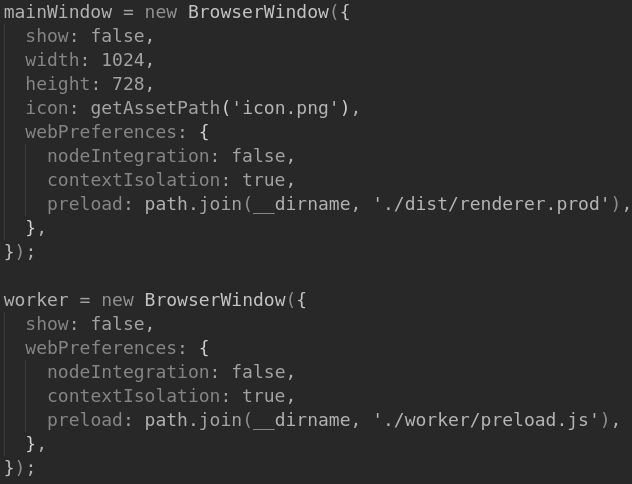
\includegraphics[height=0.3\textheight]{assets/images/practical/main+worker.png}
  \caption{Описание main- и worker-процессов приложения}
  \label{img:mainWorker}
\end{figure}

В electron-процессе указывается поведение других процессов при получении определённых событий и настраивается поведение процессов при получении событий из другого процесса. Для это используется механизм IPC - межпроцессорного взаимодействия, реализованный в Electron.

Для описания логики IPC, в Electron используется два объекта - ipcMain и ipcRenderer, которые используются в главном (electron) процессе и процессах-обработчиках (main и worker). Сообщения, посылаемые ipcRenderer и  ipcMain передаются только по указанному каналу и не могут быть получены обработчиком в другом канале.

ipcMain обрабатывает события, посылаемые процессами-обработчиками асинхронно, и может посылать сообщения процессам-обработчикам, вызывая метод webContent.send для необходимого процесса.

\begin{itemize}
  \item ipcMain.on(channel, listener) - обработчик события получения сообщения от процесса-обработчика. Вызывается при каждом новом событии;
  \item ipcMain.once(channel, listener) - обработчик события получения сообщения от процесса-обработчика. Вызывается только при первом получении события.
\end{itemize}

Пример использования ipcMain приведён на рисунке~\ref{img:ipcMain}.

\begin{figure}[H]
  \centering
  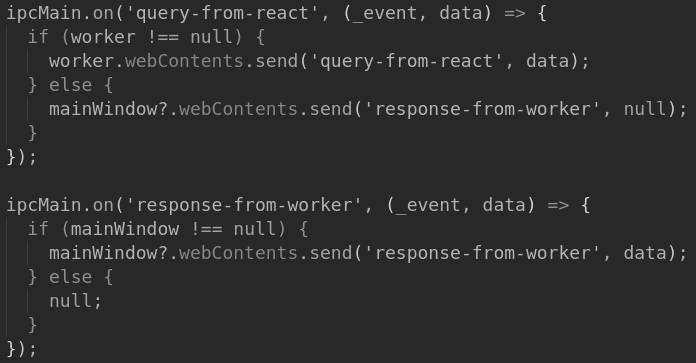
\includegraphics[height=0.2\textheight]{assets/images/practical/ipcMain.png}
  \caption{Пример использования ipcMain}
  \label{img:ipcMain}
\end{figure}

ipcRenderer предоставляет методы для получения и отправки сообщений главному процессу. Некоторые из этих методов:

\begin{itemize}
  \item ipcRenderer.on(chanel, listener) - обработчик события получения сообщения от ipcMain. Вызывается при каждом новом событии;
  \item ipcRenderer.once(chanel, listener) - обработчик события получения сообщения от ipcMain. Вызывается только при первом получении события;
  \item ipcRenderer.send(chanel, ...args) - метод, позволяющий отправлять асинхронные сообщения главному процессу. Посылаемыми данными являются args - переданные аргументы.
\end{itemize}

ipcRenderer может использоваться только в процессе-обработчике, но, так как при описании процессов-обработчиков была отключена поддержка полного набора команд, в частности команды require, необходимо указать скрипты, которые необходимо выполнить перед запуском процесса. Сделать это можно, указав в описании процесса свойство preload (предзагрузка). При этом в модуле предзагрузки доступен полный набор методов Node.js.

С помощью метода предзагрузки можно предоставить процессу-обработчику необходимые Node.js- и Electron-методы. Для этого необходимо расширить контекст этого процесса с помощью интерфейса contextBridge, который предоставляет Electron. Например, предоставить процессу-обработчику доступ к объекту ipcRenderer и методам доступа к файловой системе, можно как показано на рисунке~\ref{img:contextBridge}.

\begin{figure}[H]
  \centering
  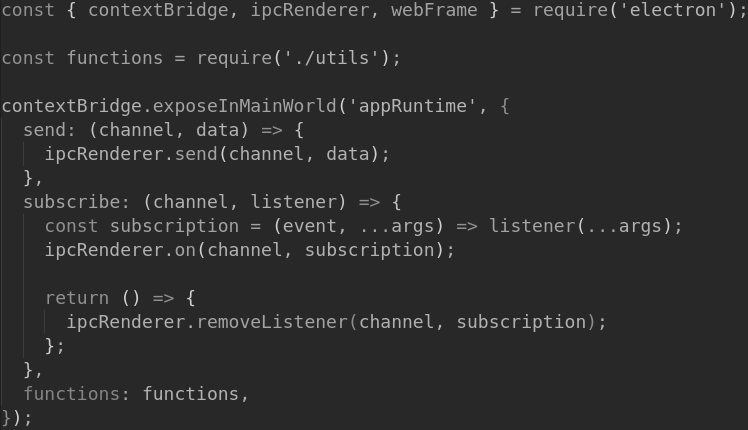
\includegraphics[height=0.2\textheight]{assets/images/practical/contextBridge.png}
  \caption{Расширение контекста процесса}
  \label{img:contextBridge}
\end{figure}

